\section{Aspectos Técnicos}

  En esta sección se desarrollan los aspectos técnicos que conforman el proyecto, incluyen la arquitectura del sistema, la estructura de la base de datos, las tecnologías utilizadas y los procesos de desarrollo e implementación. Se requerimientos realizados por el docente y las decisiones técnicas tomadas para llevar a cabo el desarrollo del sistema de gestión de productos y servicios para el restaurante. 

  \subsection{Arquitectura del Sistema}

    El sistema se basa en una arquitectura cliente-servidor, donde el cliente es una aplicación web desarrollada con el framework Astro, y el servidor es un sistema de gestión de base de datos PostgreSQL. La comunicación entre el cliente y el servidor se realiza a través de una API RESTful que permite la interacción con la base de datos para realizar operaciones CRUD (Crear, Leer, Actualizar, Eliminar) sobre los datos relacionados con clientes, personal, productos y transacciones.

    \begin{figure}[h]
      \centering
      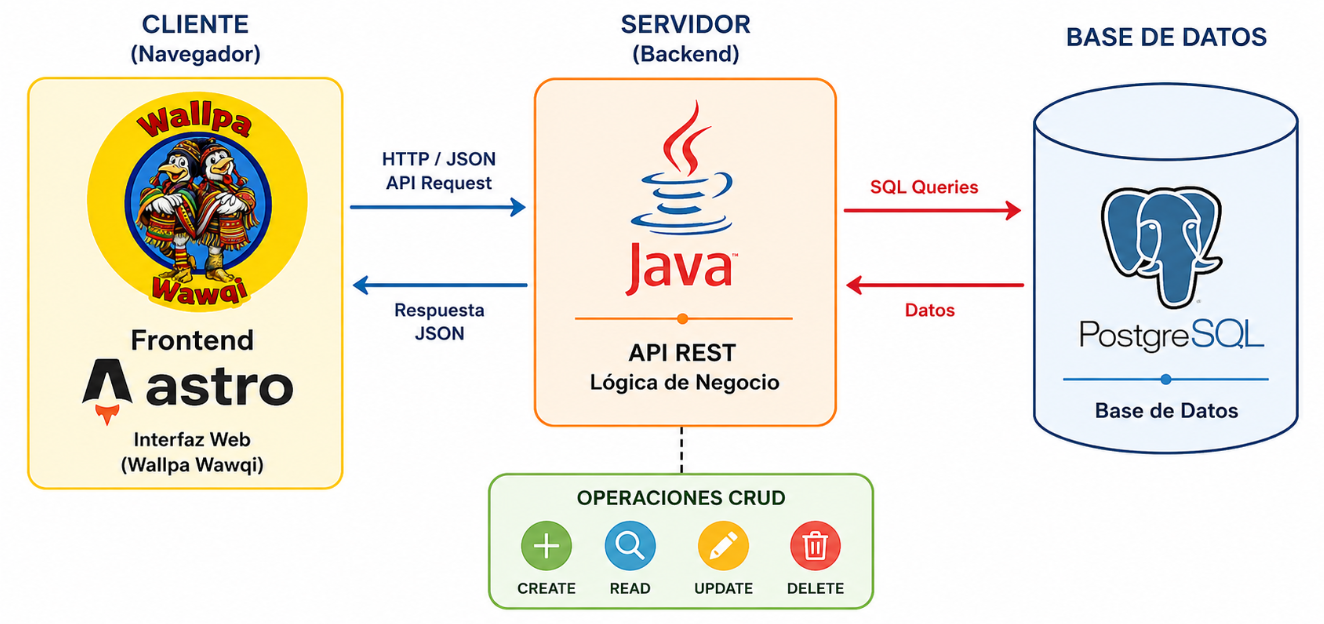
\includegraphics[width=1\textwidth]{./assets/arquitectura.png}
      \caption{Arquitectura del Sistema}
      \label{fig:arquitectura_sistema}
    \end{figure}

    \subsubsection{Frontend}

      El frontend se desarrolla utilizando el framework Astro, que permite crear interfaces web modernas y eficientes. La aplicación web proporciona una experiencia de usuario intuitiva y responsiva, facilitando la gestión de productos, clientes y transacciones. Se implementan formularios para la entrada de datos, tablas para la visualización de información y componentes interactivos para mejorar la usabilidad.

      Sobre el diseño de la interfaz, se parte de la paleta de colores creada para la identidad visual de Wallpa Wawqi además de su logo y se le agregan elemetos gráficos como íconos, botónes e imágenes para hacerla más atractiva. Dentro de las actividades realizadas para la contrucción de esta interfaz se hace uso de Figma, una herramienta de diseño de interfaces que permite crear prototipos visuales y colaborativos. A través de Figma, se diseñan las pantallas principales del sistema, incluyendo la página de inicio, el panel de administración, la gestión de productos y clientes, y la sección de transacciones. Este proceso de diseño asegura que la interfaz sea coherente con la identidad visual de la marca y que ofrezca una experiencia de usuario óptima.

      A continuación se muestra evidencia del diseño de la interfaz utilizando Figma:

      \begin{figure}[h]
        \centering
        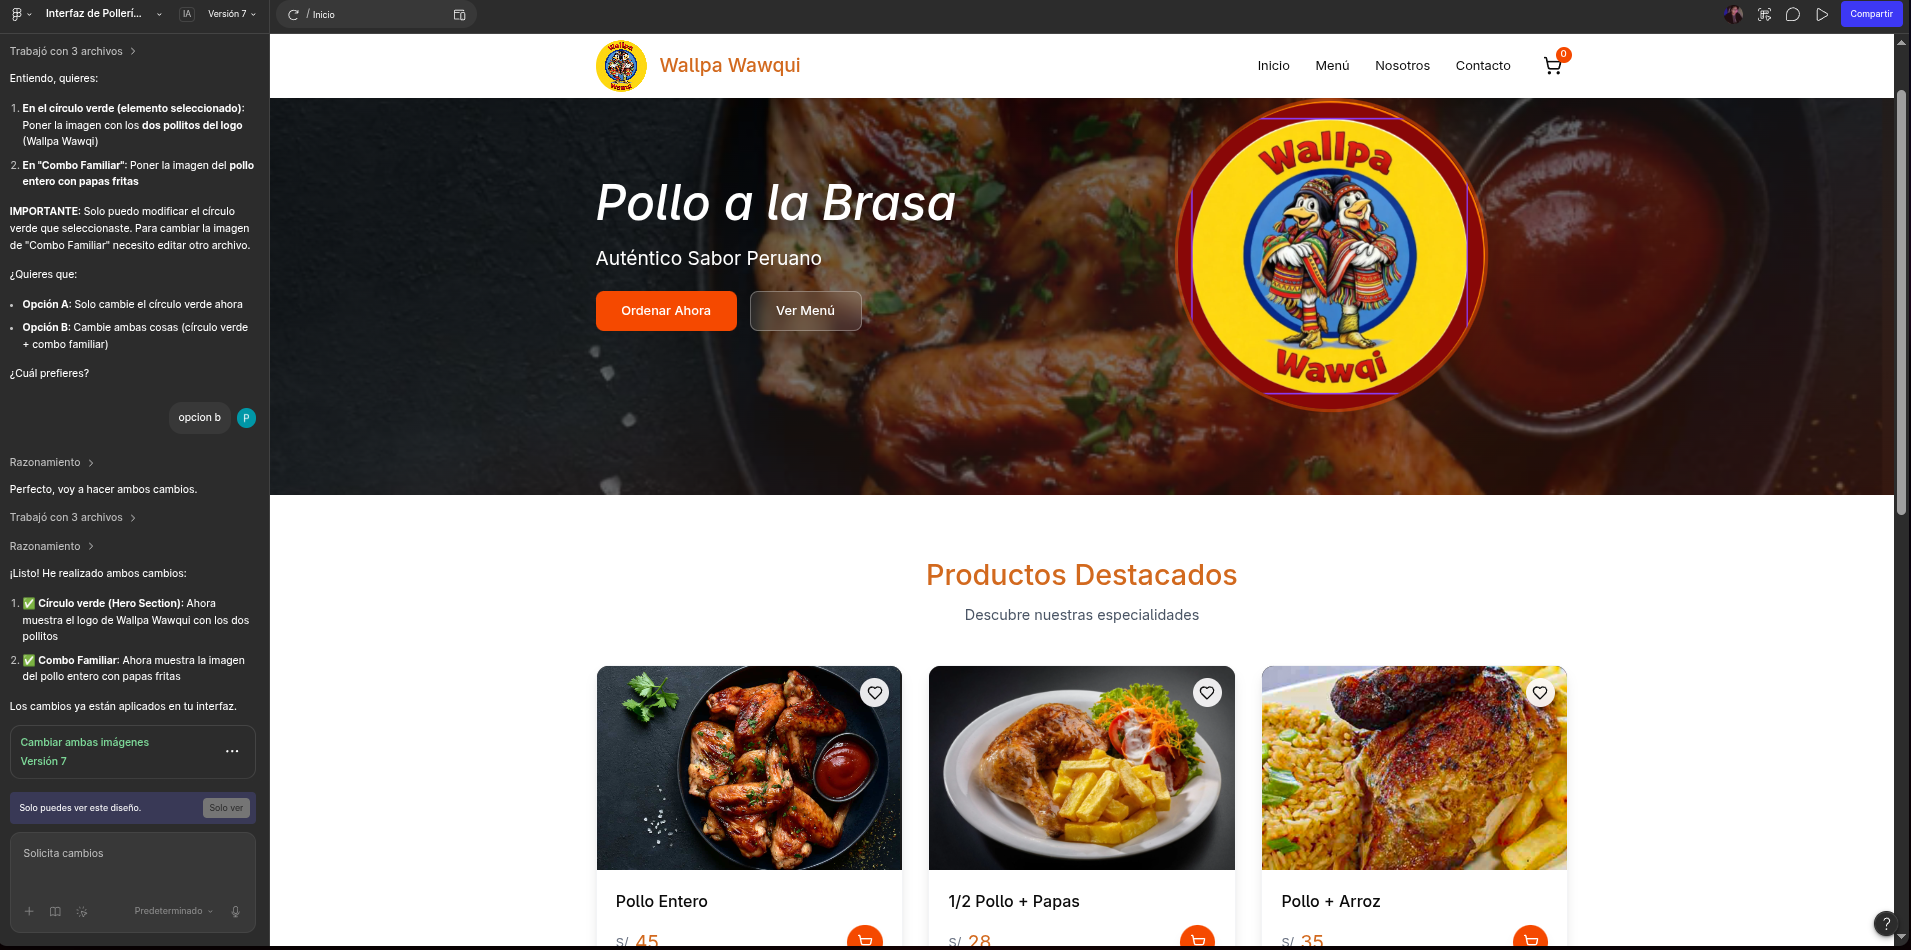
\includegraphics[width=0.8\textwidth]{./assets/figma.png}
        \caption{Diseño de la interfaz en Figma}
        \label{fig:diseño_interfaz_figma}
      \end{figure}

    \subsubsection{Backend}
      
      El backend se encarga de gestionar la lógica de negocio y la interacción con la base de datos. Se implementa una API que permita realizar operaciones sobre los datos almacenados en PostgreSQL. El backend se desarrolla utilizando Java Vanilla y se estructura en capas para separar la lógica de negocio, la capa de datos y la capa de presentación. Esto facilita el mantenimiento y la escalabilidad del sistema. Se implementan controladores para manejar las solicitudes del cliente, servicios para procesar la lógica de negocio y repositorios para interactuar con la base de datos.

      el paradigma de programación utilizado es el orientado a objetos, lo que permite organizar el código en clases y objetos que representan entidades del sistema, como clientes, productos y transacciones. Se hace uso de conceptos de este paradigma como lo es la abstracacción, herencia y polimorfismo para mejorar la modularidad y reutilización del código.

      A continuación se muestra la estrcuctura del proyecto backend:

      \begin{figure}[h]
        \centering
        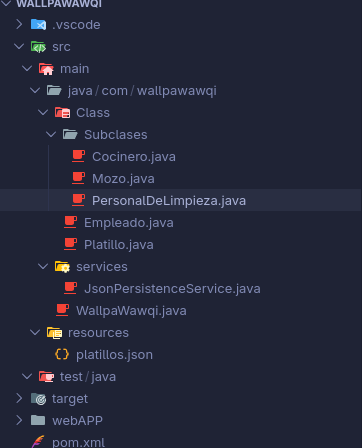
\includegraphics[width=0.35\textwidth]{./assets/estructuraProjecto.png}
        \caption{Estructura del proyecto backend}
        \label{fig:estructura_backend}
      \end{figure}

    \newpage

      Por otro lado, se muestra un fragmento del código utilizado para trabajar el objeto platillo que hace referencia a los elementos dentro de la entidad platillo que es parte de la base de datos, eso se detallará más adelante. Este código se encuentra dentro de la clase Platillo.java y se muestra a continuación:  

      \begin{listing}[H]
      \centering

      \begin{minted}[
      frame=lines,
      linenos,
      breaklines,
      fontsize=\small
      ]{java}
        
      package com.wallpawawqi.Class;

      public class Platillo {
          private long id;
          private String name;
          private double price;
          private String category;
          private String description;
          private String img;

          public long getId() { return id; }
          public void setId(long id) { this.id = id; }

          public String getName() { return name; }
          public void setName(String name) { this.name = name; }

          public double getPrice() { return price; }
          public void setPrice(double price) { this.price = price; }

          public String getCategory() { return category; }
          public void setCategory(String category) { this.category = category; }

          public String getDescription() { return description; }
          public void setDescription(String description) { this.description = description; }

          public String getImg() { return img; }
          public void setImg(String img) { this.img = img; }

          public Platillo() {
          }
      }

      \end{minted}

      \caption{Fragmento del código de la clase Platillo.java utilizado para trabajar con la entidad platillo en el backend del sistema.}
      \label{lst:codigo_modelo9}
      \end{listing}
      